

The governing equations presented in Section \ref{sec:nonlinear continuum electromechanics} are coupled by means of a suitable constitutive law. 
The objective of the following section is to introduce some notions on  constitutive laws in thermo-electro-viscoelasticity. 


\subsection{The free energy density function}

The system of PDEs presented in equations \eqref{eqn:local form conservation of linear momentum}, \eqref{eqn:Gauss law}, \eqref{eqn:Faraday} and \eqref{eqn:local form energy our format} is coupled in a nonlinear fashion through the constitutive response of the material. In the case of electro-thermo-viscoelasticity, the free energy density per unit of undeformed volume, denoted as $\Psi$, will determine the specific dependence of  $\{\vect{P},\vect{D}_0,\eta,\Dvis\}$  as functions of  $\{\vect{F},\vect{E}_0,\theta,\A\}$, where $\A=\{\vect{A}_1,\vect{A}_2,\dots,\vect{A}_{n_\text{Maxw}}\}$ represent the collection of internal variables $\vect{A}_{\alpha}$, ${\alpha} = \{1, . . . , n_\text{Maxw}\}$,
and $n_\text{Maxw}$ the number of Maxwell branches used to model the viscoelastic behaviour of the material. 
This function $\Psi$, per unit of undeformed volume, encapsulating the constitutive response of the elastic body $\mathcal{B}_0$, can be defined in terms of the deformation gradient field $\vect{F}$, the
material electric field $\vect{E}_0$, the temperature field $\theta$ and internal variables, namely
%
\begin{equation}
	\begin{aligned}
		\Psi =  \Psi\left(\vect{F},\vect{E}_0,\theta,\A\right)
	\end{aligned}
\end{equation}
%

Using thermodynamical principles, the dissipation inequality $\Dvis$ in the context of thermo-electro-viscoelasticity can be written as
%
\begin{equation}\label{eqn:disssipation1}
	\Dvis = \vect{P}:\dot{\vect{F}} - \vect{D}_0\cdot \dot{\vect{E}}_0 - \eta \dot{\theta} - \dot{\Psi}\left(\vect{F},\vect{E}_0,\theta,\A\right)\geq 0
\end{equation}
%
where the time derivative of the free energy density ${\Psi}\left(\vect{F},\vect{E}_0,\theta,\A\right)$ is computed as 
%
\begin{equation}\label{eqn:disssipation2}
	\dot{\Psi}\left(\vect{F},\vect{E}_0,\theta,\A\right)=\partial_{\vect{F}}\Psi:\dot{\vect{F}} +
	\partial_{\vect{E}_0}\Psi\cdot\dot{\vect{E}}_0 + 
	\partial_{\theta}\Psi \dot{\theta} + 
	\sum_{i={\alpha}}^{n_\text{Maxw}}\partial_{\vect{A}_{\alpha}}\Psi: \dot{\vect{A}_{\alpha}}
\end{equation}
%
assuming that the internal variables $\vect{A}_{\alpha}$ correspond second order tensors.
Use of the Coleman and Noll procedure in \eqref{eqn:disssipation1} and \eqref{eqn:disssipation2} yields the following standard constitutive relationships 
%
\begin{equation}
	\begin{aligned}
		\vect{P}\left(\vect{F},\vect{E}_0,\theta,\A\right)=\partial_{\vect{F}}\Psi; \qquad 
		%
		\vect{D}_0\left(\vect{F},\vect{E}_0,\theta,\A\right)=-\partial_{\vect{E}_0}\Psi;	\qquad
		%
		\eta\left(\vect{F},\vect{E}_0,\theta,\A\right)=-\partial_{\theta}\Psi;	
	\end{aligned}
\end{equation}
%
permitting to simplify the dissipation inequality as
%
\begin{equation}
	\Dvis\left(\vect{F},\vect{E}_0,\theta,\A\right)=-	\sum_{i={\alpha}}^{n_\text{Maxw}}\partial_{\vect{A}_{\alpha}}\Psi: \dot{\vect{A}_{\alpha}}
\end{equation}


In this section we will present the specific form of the energy density function encapsulating the constitutive coupled thermo-electro-mechanical response of the continuum $\mathcal{B}_0$, emphasising on the mathematical/physical constraints that this need to comply with.



%%%%%%%%%%%%%%%%%%%%%%%%%%%%%%%%%%%%%%%%%%%%%%%%%%%%%%%%%%%%%%%%%%%%%%%%%%%%%%%%%%%
%%%%%%%%%%%%%%%%%%%%%%%%%%%%%%%%%%%%%%%%%%%%%%%%%%%%%%%%%%%%%%%%%%%%%%%%%%%%%%%%%%%
%%%%%%%%%%%%%%%%%%%%%%%%%%%%%%%%%%%%%%%%%%%%%%%%%%%%%%%%%%%%%%%%%%%%%%%%%%%%%%%%%%%

\subsection{Thermal variation and third law of thermodynamics}
\label{sec:third_law_thermodynamics}

The Third Law of thermodynamics establishes that “the entropy of a body should be zero at Kelvin state (zero temperature)”, namely 
%
\begin{equation}
  \lim_{\theta \rightarrow 0} \eta = 0 \,.
\end{equation}

In addition, the specific heat coefficient, denoted as $c_v$ and defined as
%
\begin{equation} \label{eqn:specific_heat}
  c_v(\F,\E_0,\theta,\A) =
    -\theta \frac{\partial^2\Psi}{\partial\theta\partial\theta} =
    \theta \frac{\partial\eta}{\partial\theta}
\end{equation}
%
must be strictly positive ($c_v>0$) to ensure material stability, which implies that the free energy density $\Psi$ must be concave with respect to the temperature ($\partial^2_{\theta\theta}\Psi<0$). Furthermore, at the reference unstressed configuration, it must recover the reference specific heat coefficient $c_v^0$. 
To circumvent this and ensure strict compliance with the Third Law of Thermodynamics, we adopt the formulation recently proposed by Bonet and Gil \cite{BonetGil2026}.

In order to develop a complete constitutive model, an assumtion of independence between the thermal variation and the mechanical and electrical physics is made, which is common in the literature, considering a multiplicative decomposition as
\begin{subequations} \label{eqn:multiplicative_cv}
  \begin{equation}
    c_v(\F,\E_0,\theta,\A) = c_v^0 \X(\F,\E_0,\A) g(\theta) \,;\quad
    \X(\I,\0,\0) = 1 \,;\quad
    g(\theta_R) = 1
    \tag{\ref*{eqn:multiplicative_cv}a,b,c}
  \end{equation}
  \refstepcounter{equation}\label{eqn:multiplicative_cv_a}%
  \refstepcounter{equation}\label{eqn:multiplicative_cv_b}%
  \refstepcounter{equation}\label{eqn:multiplicative_cv_c}%
\end{subequations}
where $c_v^0$ is the specific heat coefficient at the reference configuration, $\X(\F,\E_0,\A)$ is a dimensionless function that captures the dependence of the specific heat coefficient with the mechanical and electrical physics, and $g(\theta)$ is a purely thermal function that captures the temperature dependence of the specific heat coefficient.

Later, a generalised form of the specific heat based on an additive decomposition, will be adopted to model different thermal responses or components as
\begin{subequations} \label{eqn:generalised_cv_additive}
  \begin{equation}
  c_v(\F,\E_0,\theta,\A) = \sum_{i=1}^{n} c_{v,i}^0 \X_i(\F,\E_0,\A) g_i(\theta) \, ; \qquad
    \sum_{i=1}^{n} c_{v,i}^0 \X_i(\I,\vect{0},\vect{0}) = c_v^0 \,.
  \tag{\ref*{eqn:generalised_cv_additive}a,b}
  \end{equation}
  \refstepcounter{equation}\label{eqn:generalised_cv_additive_a}%
  \refstepcounter{equation}\label{eqn:generalised_cv_additive_b}%
\end{subequations}
If such generalization is considered, Eq. \eqref{eqn:multiplicative_cv_b} should be rewritten as \eqref{eqn:generalised_cv_additive_b}.

Focusing on a single component $i$, which for simplicity, its subindex will be ommited, the integration of the specific heat coefficient in \eqref{eqn:multiplicative_cv} with respect to the temperature yields the following expression for the entropy
%Integration of the specific heat coefficient in \eqref{eqn:specific_heat} with respect to temperature after having substituted the multiplicative decomposition in \eqref{eqn:multiplicative_cv} allows to obtain the following expression for the entropy:
\begin{subequations} \label{eqn:entropy_integral}
\begin{equation}
  \eta(\F,\E_0,\theta,\A) = \eta_R(\F,\E_0,\A) G(\theta) \,;\quad
  G(\theta) = 
    \frac{1}{\xi_R}\int_{0}^{\theta} \frac{g(\vartheta)}{\vartheta} \, d\vartheta 
    % \left(
    %   1 + \frac{1}{\xi_R} \int_{0}^{\theta} \frac{g(\vartheta)}{\vartheta} \, d\vartheta
    % \right) ,
  \tag{\ref*{eqn:entropy_integral}a,b}
\end{equation}
\refstepcounter{equation}\label{eqn:entropy_integral_a}%
\refstepcounter{equation}\label{eqn:entropy_integral_b}%
\end{subequations}
with
\begin{subequations}\label{eqn:entropy_definitions}
\begin{equation}
  \eta_R(\F,\E_0,\A) = c_v^0 \X(\F,\E_0,\A)\, \xi_R
    \quad \text{and} \qquad
    \xi_R = \int_0^{\theta_R} \frac{g(\vartheta)}{\vartheta} \, d\vartheta \,,
  \tag{\ref*{eqn:entropy_definitions}a,b}
\end{equation}
\refstepcounter{equation}\label{eqn:entropy_definitions_a}%
\refstepcounter{equation}\label{eqn:entropy_definitions_b}%
\end{subequations}
where the entropy $\eta_R$ at the reference configuration is a function that bypasses the definition of $\X$ and $\xi_R$ is a scaling constant relating the entropy with the specific heat.

Analogously, subsequent integration with respect to the temperature yields the free energy density,
\begin{subequations} \label{eqn:free_energy_density_integral}
\begin{equation}
	\Psi(\F,\E_0,\theta,\A) = \Psi_K(\F,\E_0,\A) - \eta_R(\F,\E_0,\A)\,\zeta_R\,f(\theta) \,;\quad
  f(\theta) = \frac{1}{\zeta_R} \int_{0}^{\theta} G(\vartheta) \, d\vartheta \,,
  \tag{\ref*{eqn:free_energy_density_integral}a,b}
\end{equation}
\refstepcounter{equation}\label{eqn:free_energy_density_integral_a}%
\refstepcounter{equation}\label{eqn:free_energy_density_integral_b}%
\end{subequations}
with
\begin{equation} \label{eqn:free_energy_density_definitions}
    \zeta_R = \int_{0}^{\theta_R} G(\vartheta) \,d\vartheta
      = \frac{1}{\xi_R}\int_{0}^{\theta_R} g(\vartheta) \left(
        \frac{\theta}{\vartheta} -1
      \right) \, d\vartheta \,.
\end{equation}

However, the parallelism between the expressions for the entropy and the free energy density is not complete, as the free energy density includes an additional term $\Psi_K(\F,\E_0,\A)$, which is a function of the mechanical and electrical physics but independent of the temperature. This term $\Psi_K$ can be interpreted as the Kelvin state or the free energy density at zero temperature. The choice of $\Psi_K$ will be discussed in more detail in the following section, where specific expressions for the different contributions to the free energy density will be presented. Another difference with the entropy is that the scaling parameter $\zeta_R$ has units of temperature, while $\xi_R$ is dimensionless.

Finally, using terms evaluated at the reference temperature and using the partial Legendre transform, expression \eqref{eqn:free_energy_density_integral_a} can be rewritten as the following equivalent expressions,
\begin{subequations} \label{eqn:free_energy_density_integral_variant}
  \begin{equation}
    \Psi(\F,\E_0,\theta,\A) = \Psi_R(\F,\E_0,\A) - \eta_R(\F,\E_0,\A)\,\zeta_R (f(\theta) - 1) \,,
  \end{equation} \vspace{0.5pt}
  \begin{equation}
    \Psi(\F,\E_0,\theta,\A) = \Eps_R(\F,\E_0,\A) - \eta_R(\F,\E_0,\A)\,\zeta_R \left(
      f(\theta) - 1 + \frac{\theta_R}{\zeta_R}
    \right) \,.
  \end{equation}
\end{subequations}

Particular choices of the coupling functions $\Eps_R$, $\eta_R$ and $f$ will define the behaviour of each component of the material --viscoelastic and electro-mechanical-- and its thermal coupling. In the following section presents definitions of $f$ and section \ref{sec:free_energy_density_terms} presents the choices for $\Eps_R$ and $\eta_R$ defining $\Psi_R$.



\subsubsection{Thermal functions}


The triplet of functions $g_i$, $G_i$ and $f_i$ determine the thermal coupling for each physics. Once one of the three functions is specified, the remaining ones are uniquely determined via Eqs. \eqref{eqn:entropy_integral_b} and \eqref{eqn:free_energy_density_integral_b}.

However, the definition of the thermal functions is not arbitrary, as they need to comply with the mathematical and physical constraints of the model, such as the positivity of the specific heat coefficient and the satisfaction of the Third Law of Thermodynamics. For instance, considering a constant specific heat coefficient or $g(\theta)=1$ will violate the third law of Thermodynamics. In addition, they need to be flexible enough to capture different thermal responses.


\paragraph{Entropic elasticity}
Some classical models such as entropic elasticity or the thermoelasticity model for rubber in \cite{treloar1975} can be recovered by choosing the thermal functions as propsed in \cite{BonetGil2026}
\begin{subequations}
  \begin{align}
    \label{eqn:thermal_function_g_bonet}
    g_A(\theta) &= \left(\frac{\theta}{\theta_R}\right)^{\gamma} \,; \quad \gamma > 0 \\
    \label{eqn:thermal_function_f_bonet}
    f_A(\theta) &= \left(\frac{\theta}{\theta_R}\right)^{\gamma+1}
  \end{align}
\end{subequations}
where the positivity of the parameter $\gamma$ is enforced to guarantee the positivity of the specific heat coefficient.


\paragraph{Nonlinear melting}
In \cite{BonetGil2026}, integration of the $g$ function in Eq. \eqref{eqn:thermal_function_g_bonet} with appropriate constraints for the energy density yields a nonlinear melting model,
\begin{equation} \label{eqn:thermal_function_f_melting}
  f_B(\theta) = \frac{1 - \left(\frac{\theta}{\theta_M}\right)^{\gamma+1}}
                     {1 - \left(\frac{\theta_R}{\theta_M}\right)^{\gamma+1}}
\end{equation}
where $\theta_M$ is a parameter governing the melting temperature of the material, at which the free energy density vanishes.


\paragraph{Nonlinear softening}
In this work, when considering the additive decomposition of the free energy density following Eq. \eqref{eqn:generalised_cv_additive}, the authors have been observed in section \ref{sec:calibration} the need to consider some other behaviours for specific components of the material, such as a nonlinear softening being convex with respect to the temperature. Convexity of the free energy density with respect to the temperature is a property that calls into doubt the positivity of the specific heat coefficient. However, the physical constraints need to be evaluated after the specific choices for each term of the free energy density in \ref{sec:free_energy_density_terms} and will be analysed in SECTION.
The scaling of the energy density is based on a modified Weibull distribution of the form
\begin{equation}
  u(\theta) = \exp\left(-\left(\frac{\theta}{\theta_T}\right)^{\gamma+1}\right) ; \quad \gamma > 0 \,,
\end{equation}
where $\theta_T$ is a parameter governing the transition temperature of the material properties. The function $f$ is then defined as a scaled and shifted version of $u$ as
\begin{equation} \label{eqn:thermal_function_f_softening}
  f_C(\theta) = \frac{(1-\delta)\, u(\theta) + \delta}{(1-\delta)\, u(\theta_R) + \delta} \,; \quad \delta \in (0,1) \,,
\end{equation}


\begin{figure}[htb]
  \centering
  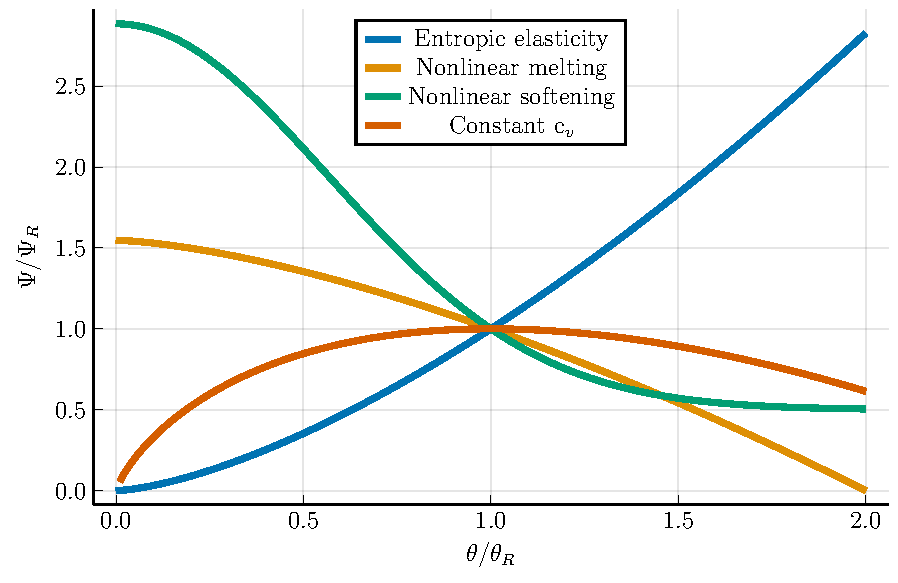
\includegraphics[width=0.6\textwidth]{figures/thermal_functions.pdf}
  \caption{Qualitative comparison of functions $f_i$ controlling the material responses of the free energy density with respect to the temperature.}
  \label{fig:comparison_thermal_laws_f}
\end{figure}

Figure \ref{fig:comparison_thermal_laws_f} shows a comparison of the different thermal functions $f_i$ presented in this section, which will be used in the later section \ref{sec:calibration} to capture different thermal responses of the material. The flexibility of the formulation allows to capture different behaviours, such as the nonlinear softening behaviour shown by function $f_C$.


% \begin{tcolorbox}
%   NOTE: $\;G = \zeta_R\,f' \;;\quad g = \theta\xi_R\,G'$ \newline
%   The implementation in HyperFEM is as follows:
%   \begin{align*}
%     C &= (1-\delta) u(\theta_R) + \delta \\
%     f &= \frac{(1-\delta) u(\theta) + \delta}{C} \\
%     f' &= -\frac{1-\delta}{C}\frac{\gamma+1}{\theta_T}\left(\frac{\theta}{\theta_R}\right)^{\gamma} u(\theta) \\
%     f'' &= \frac{1-\delta}{C}\frac{\gamma+1}{\theta^2}\left(\frac{\theta}{\theta_R}\right)^{\gamma+1}
%       \left((\gamma+1) \left(\frac{\theta}{\theta_T}\right)^{\gamma+1}-\gamma\right) u(\theta)
%   \end{align*}
% \end{tcolorbox}






%%%%%%%%%%%%%%%%%%%%%%%%%%%%%%%%%%%%%%%%%%%%%%%%%%%%%%%%%%%%%%%%%%%%%%%%%%%%%%%%%%%
%%%%%%%%%%%%%%%%%%%%%%%%%%%%%%%%%%%%%%%%%%%%%%%%%%%%%%%%%%%%%%%%%%%%%%%%%%%%%%%%%%%
%%%%%%%%%%%%%%%%%%%%%%%%%%%%%%%%%%%%%%%%%%%%%%%%%%%%%%%%%%%%%%%%%%%%%%%%%%%%%%%%%%%


\subsection{Free energy density decomposition}
\label{sec:free_energy_density_terms}

On section \ref{sec:third_law_thermodynamics}, the thermal variation of the free energy density has been uncoupled from the mechanical and electrical physics via a multiplicative decomposition in Eq. \eqref{eqn:multiplicative_cv}. Considering the additive decomposition of the specific heat coefficient in Eq. \eqref{eqn:generalised_cv_additive} it can be can be propagated to the free energy density, namely, volumetric and isochoric contributions $\bar\Psi$ and $\hat\Psi$.
Additional physics such as electro-mechanical coupling denoted as $\Psi_\epsilon$ can be straightforwardly added as an additional term, reading
\begin{equation} \label{eqn:free_energy_density_additive}
	\Psi(\F,\E_0,\theta,\A) = \bar\Psi(J,\theta) + \hat\Psi(\F,\theta,\A) + \Psi_{\epsilon}(\F,\E_0,\theta) \,.
\end{equation}

The reader would note that each component of the free energy density $\Psi_i \in \{\bar\Psi, \hat\Psi, \Psi_\epsilon\}$ in \eqref{eqn:free_energy_density_additive} follows the definition in \eqref{eqn:free_energy_density_integral_variant}, thus, it depends on the internal energy at the reference configuration $\Eps_{R_i}$, the reference entropy $\eta_{R_i}$ and the corresponding thermal coupling function $f_i$. The following sections will propose specific choices and, for the sake of completeness, the uncoupled version of \eqref{eqn:free_energy_density_additive} is displayed below,
%The following sections will present the specific definitions for the free energy density at reference configuration and the corresponding thermal coupling for each component. For the sake of completeness, the uncoupled version of Eq. \eqref{eqn:free_energy_density_additive} is shown as below,
\begin{multline} \label{eqn:full_free_energy_density_model}
	\Psi(\F,\E_0,\theta,\A) =
	\underbrace{%
		\bar\Psi_R(J) - \bar\eta_R(J) \bar\zeta_R \left(\bar f(\theta)-1\right) \vphantom{\frac{A}{B}}%
	}_{\bar\Psi} + \\ +
    \underbrace{%
		\hat\Psi_{R,\infty}(\F) \hat f_\infty(\theta) + \sum_\alpha^{n_\text{Maxw}} \hat\Psi_{R,\alpha}(\F,\Aa) \hat f_\alpha(\theta)%
	}_{\hat\Psi} +
	\underbrace{%
		\Psi_{R,\epsilon}(\F,\E_0) f_\epsilon(\theta) \vphantom{\sum_{a}^{n_M}}%
	}_{\Psi_\epsilon} .
\end{multline}
%
%where the choices in sections \ref{sec:volumetric_model}, \ref{sec:viscoelastic_model} and \ref{sec:electro_mech_model} have been substituted, yielding \eqref{eqn:full_free_energy_density_model}.



\subsubsection{Volumetric free energy density} \label{sec:volumetric_model}

The pair of functions $\Eps_R$ and $\eta_R$ in \eqref{eqn:free_energy_density_integral_variant} must be convex and concave functions as  reported in \cite{BonetGil2026} to satisfy stability conditions,
\begin{align}
  \label{eqn:volumetric_eta}
	\bar\eta_R(J) &= c_v^0\bar\xi_R + c_v^0\Gamma\frac{J^q-1}{q} \,, \\
  \label{eqn:volumetric_Epsilon}
	\bar\Eps_R(J) &= U(J) + \beta(J-1) + \bar\Eps_0 \,; \quad U(J) = \frac{1}{2}\kappa_R(J-1)^2 \,,
\end{align}
where $\Gamma$ is the Mie-Grüneisen constant, $q$ is a dimensionless parameter, and the volumetric energy contribution $U$ could be replaced by other \emph{coercive} term having the bulk modulus $\kappa_R$ as tangent for $J=1$. The reference value $\bar\Eps_0$ is a constant that guarantees positiveness of the free energy density and it takes a minimum value of $c_v^0 \bar\xi_R \theta_R$.
The parameter $\beta$ is related with the Mie-Grüneisen constant $\Gamma$ by imposing null pressure at the reference configuration,
\begin{equation}
	\left.\frac{\partial\bar\Psi}{\partial J}\right|_{\substack{J=1\hfill\\ \theta=\theta_R}} = 0 \ \Longleftrightarrow \
		\beta = \Gamma c_v^0 \theta_R \,.
\end{equation}
The parameter Mie-Grüneisen can also been related with the linear thermal expansion coefficient with the relation
\begin{equation}
	\left.\frac{\partial^2\bar\Psi}{\partial J \partial \theta}\right|_{\substack{J=1\hfill\\ \theta=\theta_R}} =
		-3\alpha\kappa_R = -\Gamma c_v^0 \,.
\end{equation}

Following the proposal in \cite{BonetGil2026}, the thermal function $\bar f$ considered for the volumetric part corresponds to the entropic elasticity in Eq. \eqref{eqn:thermal_function_f_bonet}, which ensures the positivity of the specific heat coefficient for the volumetric part.
For the particular case $q=1$, the volumetric free energy density would read
\begin{equation} \label{eqn:volumetric_free_energy}
  \bar\Psi(J) = 
    \underbrace{U(J) \vphantom{\frac{c_v^0}{\bar\gamma}}}_{\bar\Psi_R} -
    \underbrace{\left(\frac{c_v^0}{\bar\gamma} + 3\alpha\kappa_R(J-1)\right)}_{\bar\eta_R}
    \underbrace{{\frac{\theta_R}{\bar\gamma+1}}}_{\bar\zeta_R}
    \left( \vphantom{\frac{c_v^0}{\bar\gamma}} \right.
      \underbrace{\left(\frac{\theta}{\theta_R}\right)^{\bar\gamma+1}}_{\bar f} -1
    \left. \vphantom{\frac{c_v^0}{\bar\gamma}} \right) .
\end{equation}



\subsubsection{Isochoric free energy density} \label{sec:viscoelastic_model}

The simple choice $\hat\Psi_R = -\hat\zeta_R\hat\eta_R$ implies the assumption that the deviatoric free energy density at the Kelvin state is null, $\hat\Psi_K=0$, as well as null contribution to the specific heat coefficient at the reference configuration, $\hat{c}_v(\I,\theta_R)=0$, allowing further simplification of Eqs. \eqref{eqn:free_energy_density_integral} and \eqref{eqn:free_energy_density_integral_variant}. Additionally, the consideration of a generalized Maxwell model will split the deviatoric free energy density $\hat\Psi$ into a long-term component $\hat\Psi_\infty$ and a set of viscous branches $\hat\Psi_\alpha$. Both assumptions will allow to rewrite the deviatoric component in \eqref{eqn:free_energy_density_additive} as
% \begin{equation}
%   \label{eqn:isochoric_thermal_coupling}
% 	\hat\Psi(\F,\theta,\A) = \hat\Psi_R(\F,\A) \hat f(\theta) \,,
% \end{equation}
% which facilitates using standard constitutive models from literature.
% Notice that the inner product in \ref{eqn:isochoric_thermal_coupling} implies consistent definitions for the thermal coupling of each component of the free energy density, such as a generalized Maxwell model for viscoelasticity,
\begin{equation}
  \label{eqn:isochoric_maxwell_decomposition}
  \hat\Psi(\F,\theta,\A) = \hat{\Psi}_{R,\infty}(\F) \hat{f}_\infty(\theta) +
	\sum_{\alpha=1}^{n_\text{Maxw}} \hat{\Psi}_{R,\alpha}(\F,\Aa) \hat{f}_\alpha(\theta) \,.
\end{equation}%
Notice that the definition in \eqref{eqn:generalised_cv_additive} implies the definition of a thermal coupling function for each component of the free energy density.

\begin{figure}[htb]
	\centering
	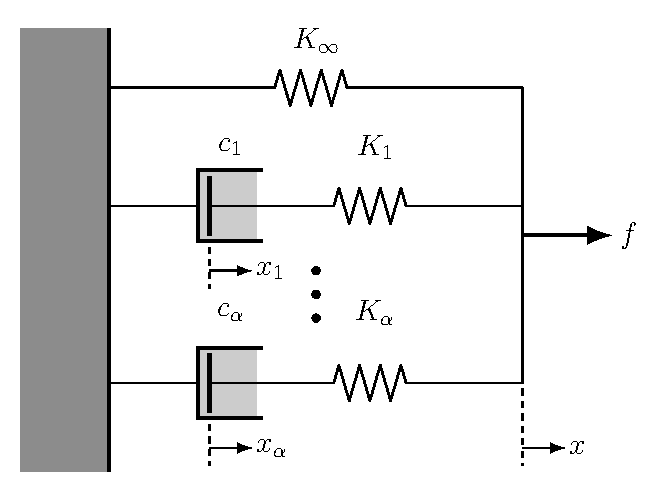
\includegraphics[width=0.5\linewidth]{figures/one_dim_maxwell.pdf}
	\caption{One-dimensional Maxwell model.}
	\label{fig:one_dim_maxwell}
\end{figure}


In this work, a non-linear Mooney-Rivlin model will be considered for the long-term component
\begin{equation}
  \label{eqn:isochoric_mooney_rivlin}
	\hat\Psi_{R,\infty}(\F) =
		\frac{\mu_1}{2\alpha_1 3^{(\alpha_1-1)}}((\hat\F\!:\!\hat\F)^{\alpha_1} - 3^{\alpha_1}) +
		\frac{\mu_2}{2\alpha_2 3^{(\alpha_2-1)}}((\hat\H\!:\!\hat\H)^{\alpha_2} - 3^{\alpha_2}) \,,
\end{equation}
where the isochoric deformation gradient and the cofactor are defined as follow,
\begin{equation}
  \hat\F = J^{-\sfrac{1}{3}}\F \,; \qquad \hat\H = J^{-\sfrac{2}{3}}\H \,.
\end{equation}
In the later section \ref{sec:calibration} the choice of this model will be discussed, which is motivated by the dependence on the invariant of $\hat\H$.

With regard to the viscous contributions $\hat\Psi_{R_\alpha}$, these depend on an intermediate elastic state $\F_{\mathrm{e}_{\alpha}}$ as schematically depicted in \ref{fig:one_dim_maxwell}. Following the one-dimensional Maxwell model shown in \ref{fig:one_dim_maxwell}, the rate change of each intermediate state or internal variable is given the simple one-dimensional evolution law
%
%As for the viscous contributions $\hat\Psi_{R,\alpha}$, these are based on the evolution of internal state variables $\A$. A schematic one-dimensional version of the internal state variables is shown in figure \ref{fig:one_dim_maxwell}, where the one-dimensional evolution law is given by
%
\begin{equation}
  \label{eqn:one-dim_evolution_law}
  \left.\frac{\mathrm{d}f_\alpha}{\mathrm{d}t}\right|_{x=\text{const}} = \frac{1}{\tau_\alpha} f_\alpha\,.
\end{equation}
%
The extension to the three-dimensional case will be described in section \ref{sec:incompressible_viscoelasticity}, where the finite strain viscoelasticity model and the associated evolution laws are based on a multiplicative decomposition of the deformation gradient, designed to guarantee positive viscous dissipation and comply with the second law of thermodynamics, allowing to define the elastic strain $\F_{\mathrm{e}_\alpha}$ in terms of $\F$ and the internal state variables $\Aa$.
%
Once there is a consistent definition of viscous strain, the stresses can be evaluated by a standard constitutive model, such as a neo-Hookean model,
\begin{equation}
  \label{eqn:isochoric_visco_neo_hokean}
  \hat\Psi_{R,\alpha}(\F,\Aa) = \frac{\mu_\alpha}{2} \left(
    \hat\F_{e_\alpha}\!:\!\hat\F_{e_\alpha} - 3
  \right) .
\end{equation}


Finally, the choice of the thermal laws is justified by evidence of experimental data in Section \ref{sec:calibration}, where the elastic part has proven to be very stable for the tested range of temperatures, while the viscous properties exhibit an abrupt change. The nonlinear melting \eqref{eqn:thermal_function_f_melting} which is a soft function has been used for the long term component, and the nonlinear softening \eqref{eqn:thermal_function_f_softening} has been used for the viscoelastic components.



\subsubsection{Electro-mechanical coupling} \label{sec:electro_mech_model}

Finally, the electro-mechanical coupling term $\Psi_{\epsilon}$ is essential for modelling the behaviour of Electro-Active Polymers (EAPs). In these materials, the electric state interacts with mechanical deformation, potentially inducing significant thermal fluctuations.
The same hypothesis in \ref{sec:viscoelastic_model} holds, then, the thermal variation of the free energy density in \eqref{eqn:free_energy_density_integral_variant} is simplified as
\begin{equation} \label{eqn:electro_mech_copupling}
  \Psi(\F,\E_0,\theta) = \Psi_{R,\epsilon}(\F,\E_0) f_\epsilon(\theta) \,.
\end{equation}
The purely electro-mechanical energy follows the commonly expression used in XXXXX,
% The use of polyconvex thermodynamic potentials in this part of the model is crucial to ensure numerical stability and the physical realism of the solutions in large strain regimes.
\begin{equation} \label{eqn:electro_mech_coupling_ref}
	\Psi_{R,\epsilon}(\F,\E_0) = -\frac{\varepsilon_r \varepsilon_0}{2J}\H\E_0 \cdot \H\E_0 \,,
\end{equation}
where $\varepsilon_0$ is the vacuum permittivity and $\varepsilon_r$ is the relative permittivity of the material. The thermal coupling function $f_\epsilon$ will be defined in the later section \ref{sec:calibration} based on experimental evidence, which shows a smooth change in the electro-mechanical coupling with temperature.



%%%%%%%%%%%%%%%%%%%%%%%%%%%%%%%%%%%%%%%%%%%%%%%%%%%%%%%%%%%%%%%%%%%%%%%%%%%%%%%%%%%
%%%%%%%%%%%%%%%%%%%%%%%%%%%%%%%%%%%%%%%%%%%%%%%%%%%%%%%%%%%%%%%%%%%%%%%%%%%%%%%%%%%
%%%%%%%%%%%%%%%%%%%%%%%%%%%%%%%%%%%%%%%%%%%%%%%%%%%%%%%%%%%%%%%%%%%%%%%%%%%%%%%%%%%


\subsection{Incompressible viscoelasticity at finite strains}
\label{sec:incompressible_viscoelasticity}

This Section presents a theoretical framework for large strain compressible viscoelasticity, where  the viscous deformation is not assumed isochoric at a first instance.

\subsubsection{Continuum kinematics and multiplicative decomposition}
\label{sec:viscous_kinematics_multiplicative}

\begin{figure}
	\centering
	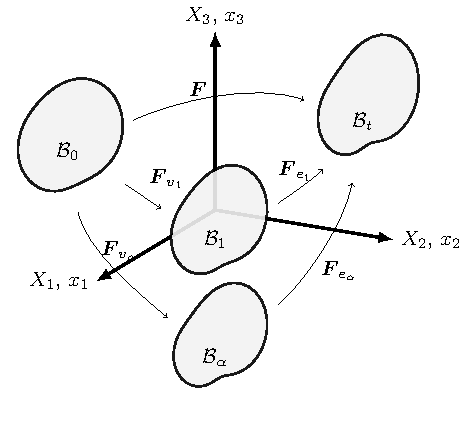
\includegraphics[width=0.5\linewidth]{figures/multiplicative_decomposition.pdf}
	\caption{Multiplicative decomposition of the deformation gradient.}
	\label{fig:2split}
\end{figure}


Viscoelasticity in finite strains using a generlized three dimensional Maxwell model is typically formulated using a multiplicative decomposition of the deformation gradient tensor $\vect{F}$ in terms of its elastic and viscous components
\cite{Kroner1959, Lee1969elastic, Anand1985constitutive, Bergstrom1998}
%
\begin{equation}\label{eqn:multiplicative_F}
	\F = \F_{\mathrm{e}_\alpha} \F_{\mathrm{v}_\alpha},
\end{equation}
%
through the introduction of suitable intermediate (i.e. stress free) configurations (see Fig.~\ref{fig:2split}). As it is illustrated, the number of viscous elements $\alpha=1\ldots n_{\alpha}$ in this generalised Maxwell model can be arbitrary. Note that $\F_{\mathrm{v}_\alpha}$ denotes the internal variable of the corresponding viscous element $\alpha$ that determines the current state of the system, with thermo-dynamical equilibrium achieved when $\F_{\mathrm{v}_\alpha} = \F$. Moreover, to ensure that the proposed constitutive model is objective (i.e. frame invariant), suitable rotation free right Cauchy-Green deformation tensors can be defined as
%
\begin{subequations}
	\label{eqn:Cauchy-Green}
	\begin{equation}
    \C = \F^{\mathrm{T}} \F \,;\quad
    \C_{\mathrm{v}_\alpha}=\F^{\mathrm{T}}_{\mathrm{v}_\alpha} \F_{\mathrm{v}_\alpha} \,,
    \tag{\ref*{eqn:Cauchy-Green}a,b}
	\end{equation}
  \refstepcounter{equation}\label{eqn:Cauchy-Creen_a}%
  \refstepcounter{equation}\label{eqn:Cauchy-Creen_b}%
\end{subequations}
%
where $\C$ and $\C_{\mathrm{v}_\alpha}$ denote the total and viscous right Cauchy-Green deformation tensors, respectively. It should be pointed out that unlike $\C$ and $\C_{\mathrm{v}_\alpha}$, the right Cauchy-Green deformation tensor $\C_{\mathrm{e}_\alpha}=\F^{\mathrm{T}}_{\mathrm{e}_\alpha} \F_{\mathrm{e}_\alpha}$ is not defined in the reference configuration, but at the intermediate (elastic free) configuration and, as such, it is not rotation free. Indeed, the multiplicative decomposition of the deformation gradient \eqref{eqn:multiplicative_F} has an internal redundant rotation, which means $\F$ can equally be written as
%
\begin{equation}
	\label{eqn:F_defcomposition}
	\F=\F_{\mathrm{e}_\alpha}^{*}  \F_{\mathrm{v}_\alpha}^{*} \quad \text{with} \quad \F_{\mathrm{v}_\alpha}^{*} = \boldsymbol{Q} \F_{\mathrm{v}_\alpha} \quad \text{and} \quad \F_{\mathrm{e}_\alpha}^{*} = \F_{\mathrm{e}_\alpha}  \boldsymbol{Q}^{\mathrm{T}},
\end{equation}
%
where $\boldsymbol{Q} \in \text{SO}(3)$ denotes an arbitrary rotation tensor. Following a similar idea to that of \Red{Reference \cite{Holthusen2023},5} in this paper we propose to eliminate this redundant rotation by selecting $\boldsymbol{Q}$ as $\boldsymbol{R}_{\mathrm{v}_\alpha}^{\mathrm{T}}$, namely, the rotation tensor emanating from the right polar decomposition of the viscous deformation gradient tensor 
$\F_{\mathrm{v}_\alpha}=	 \boldsymbol{R}_{\mathrm{v}_\alpha}  \boldsymbol{U}_{\mathrm{v}_\alpha}$. Hence, a unique multiplicative decomposition of the deformation gradient $\F$ can then be obtained as
%
\begin{equation}
	\label{eqb:Fv_rotation_free}
	\F = \F_{\mathrm{e}_\alpha}^{*}  \boldsymbol{U}_{\mathrm{v}_\alpha}, \quad \F_{\mathrm{e}_\alpha}^{*} = \F_{\mathrm{e}_\alpha} \boldsymbol{R}_{\mathrm{v}_\alpha},
\end{equation}
%
whereby 
%
\begin{equation}
  \label{eqn:Cea}
	\C_{\mathrm{e}_\alpha} = \F_{\mathrm{e}_\alpha}^{*\mathrm{T}} \F_{\mathrm{e}_\alpha}^{*}=\boldsymbol{U}_{\mathrm{v}_\alpha}^{-1} \C \boldsymbol{U}_{\mathrm{v}_\alpha}^{-1},
\end{equation}
%
and the symmetric viscous strain tensor $\boldsymbol{U}_{\mathrm{v}_\alpha}$ is also uniquely defined. 


\subsubsection{Strain energy function}
\label{sec:strain_energy_function}

To guarantee that $\Psi_\alpha$ vanishes when $\boldsymbol{U}_{\mathrm{v}_\alpha}$ and $\F$ only differ by a rigid body rotation (i.e. thermo-dynamical equilibrium), \cite{Liu2025} particularise the definition of $\Psi_\alpha$  as 
%
\begin{equation}
	\label{eqn:Psi_Cea}
	\hat\Psi_\alpha(\F,\Aa) =
	\widetilde\Psi_\alpha(\C,\U_{\mathrm{v}_{\alpha}}) =
	\widetilde\Psi_{\mathrm{e}_{\alpha}}(\C_{\mathrm{e}_\alpha})
\end{equation}
%
where $\C_{\mathrm{e}_\alpha}$ is defined in \eqref{eqn:Cea} and the symbol $\widetilde{\Psi}$ is used to emphasise the alternative functional dependency. Moreover, for the particular case of isotropic viscoelasticity, the strain energy contributions $\Psi_{\infty}(\C)$ and $\widetilde{\Psi}_{\alpha}(\C_{\textrm{e}_\alpha})$ can be particularised in terms of their respective invariants $\{I_{\bullet},II_{\bullet},III_{\bullet}\}$, which will be implicitly assumed in what follows. Note that extension to the anisotropic case would imply the incorporation of structural tensors representative of their appropriate symmetry groups as further arguments of the strain energy density, which were presented in \cite{Liu2025}.



\subsubsection{First and second Piola-Kirchhoff stress tensor}
\label{sec:visco_first_second_Piola}

The first Piola-Kirchhoff stress tensor $\P$ can be obtained from the directional derivative of the strain energy $\Psi$ in Eq. \eqref{eqn:full_free_energy_density_model} with respect to $\F$ wilst holding the internal state variable $\vect{U}_{\textrm{v}_{\alpha}}$ constant (i.e. $D\left.\Psi\right|_{\vect{U}_{\mathrm{v}_{\alpha}}=\text{const}}[\delta\F] = \P:\delta\F$) to yield
%
\begin{subequations}
  \label{eqn:visco_first_piola}
  \begin{equation}
    \P = \frac{\partial\Psi}{\partial\F} = \bar\P + \hat\P_\infty + \sum_{\alpha}\hat\P_\alpha + \P_\epsilon
  \end{equation}
  \begin{equation}
    \bar\P = \frac{\partial\bar\Psi}{\partial\F} = \frac{\partial\bar\Psi}{\partial J}\I = p\I \,,\quad
    \hat\P_\infty = \frac{\partial\hat\Psi_\infty}{\partial\F} \,,\quad
    \hat\P_\alpha = \left.\frac{\partial\hat\Psi_\alpha}{\partial\F}\right|_{\vect{U}_{\mathrm{v}_{\alpha}}=\text{const}} \,,\quad
    \P_\epsilon = \frac{\partial\Psi_\epsilon}{\partial\F} \,,
  \end{equation}
\end{subequations}
%
where $\bar\P$ is the volumetric pressure tensor, $\hat\P_\infty$ is the long-term stress tensor, $\hat\P_\alpha$ denotes the viscous stress tensor of the corresponding Maxwell element and the term $\P_\epsilon$ is the dielectric stress tensor. The symbol $\left.(\bullet)\right|_{\boldsymbol{U}_{\textrm{v}_{\alpha}}=\textrm{const}}$ emphasises that the internal state variable $\boldsymbol{U}_{\textrm{v}_{\alpha}}$ is held constant.

There is a fundamental relation between the first and the second Piola-Kirchhoff stress tensors.
For consistency with the previous publication \cite{Liu2025}, the second rather than the first Piola-Kirchhoff stress tensor will be employed for the viscous stressess, noting that the first Piola-Kirchhoff stress tensor can easily recovered as $\P=\F\S$ from Eq. \eqref{eqn:Cauchy-Creen_a}.


Thus, the second Piola-Kirchhoff stress tensor $\boldsymbol{S}$ can now be obtained from the directional derivative of the strain energy $\Psi$ with respect to a perturbation $\delta \C$ whilst holding the internal state variable $\boldsymbol{U}_{\textrm{v}_{\alpha}}$ constant (i.e. $D\left.\Psi\right|_{\boldsymbol{U}_{\textrm{v}_{\alpha}}=\textrm{const}}[\delta \C]=\boldsymbol{S}:\frac{1}{2}\delta \C$). Focusing on a single viscous Maxwell element,
%
\begin{equation}
	\label{eqn:maxw_Sa}
	\boldsymbol{S}_\alpha = 2 \left.\frac{\partial \Psi_\alpha}{\partial \C}\right|_{\boldsymbol{U}_{\textrm{v}_{\alpha}}=\textrm{const}}.
\end{equation}
%
Note that from \eqref{eqn:Psi_Cea} and the definition \eqref{eqn:Cea}, the viscous stress tensor $\boldsymbol{S}_\alpha$ will vanish when $\boldsymbol{U}_{\mathrm{v}_\alpha}$ only differs from $\F$ by a rigid body rotation. For the subsequent derivation, the elastic second Piola-Kirchhoff stress tensor of the viscous Maxwell element $\boldsymbol{S}_{\mathrm{e}_\alpha}$ is defined as
%
\begin{equation}
	\label{eqn:maxw_Sea}
	\boldsymbol{S}_{\mathrm{e}_\alpha} = 2\frac{\partial \widetilde{\Psi}_{\alpha}\left(\C_{\mathrm{e}_\alpha} \right)}{\partial \C_{\mathrm{e}_\alpha}}.
\end{equation}
%
It is now useful to relate stress $\boldsymbol{S}_\alpha$ \eqref{eqn:maxw_Sa}$_c$ to stress $\boldsymbol{S}_{\mathrm{e}_\alpha}$ \eqref{eqn:maxw_Sea} by noticing that
%
\begin{equation}\label{eqn:Sea_Sa}
	D\left.\Psi_{\alpha}\right|_{\boldsymbol{U}_{\textrm{v}_{\alpha}}=\textrm{const}}[\delta \C]=D \widetilde{\Psi}_{\alpha}[D\left.\C_{\textrm{e}_{\alpha}}\right|_{\boldsymbol{U}_{\textrm{v}_{\alpha}}=\textrm{const}}[\delta \C]],
\end{equation}
%
and substituting the directional derivative of \eqref{eqn:Cea} with respect to $\delta \C$ into \eqref{eqn:Sea_Sa} results in
%
\begin{equation}
	\label{eqn:Sea_Uva}
	\boldsymbol{S}_{\mathrm{e}_\alpha} = \boldsymbol{U}_{\mathrm{v}_\alpha}  \boldsymbol{S}_{\alpha}  \boldsymbol{U}_{\mathrm{v}_\alpha},
\end{equation}
%
which establishes a necessary relationship between the Maxwell viscous contribution to the second Piola-Kirchhoff stress tensor and its elastic counterpart.



\subsubsection{Volume-preserving constraints}
\label{sec:volume-preserving_constraints}

Incompressibility of the viscous stretch contribution $\boldsymbol{U}_{\mathrm{v}_{\alpha}}$ implies that $\text{det}\boldsymbol{U}_{\mathrm{v}_{\alpha}} = 1$ or, alternatively, by recalling \eqref{eqn:multiplicative_F}, that
%
\begin{equation}
	\label{eqn:visco_Je}
	J_{\mathrm{e}_{\alpha}} = \text{det}\F_{\mathrm{e}_{\alpha}}= \text{det}\F = J. 
\end{equation}
%
Time differentiation of above kinematic constraint \eqref{eqn:visco_Je} leads to 
%
\begin{equation}
	\label{eqn:visco_Je_t}
	\C_{\mathrm{e}_{\alpha}}^{-1} : \left.\frac{\mathrm{d}\C_{\mathrm{e}_{\alpha}} }{\mathrm{d}t} \right|_{\F=\text{const}} = 0,
\end{equation}
%
which arises as a kinematic constraint for the time evolution of the elastic right Cauchy-Green tensor $\C_{\textrm{e}_{\alpha}}$. Correspondingly, the Maxwell strain energy density $\Psi_\alpha$ must be defined to only penalise distortional contributions, that is
%
\begin{subequations}
  \label{eqn:isochoric_Psi_Cea}
  \begin{equation}
    \Psi_\alpha (\C,~\boldsymbol{U}_{\mathrm{v}_{\alpha}}) = 
      \hat{\widetilde{\Psi}}_\alpha\left( \C_{\mathrm{e}_{\alpha}}\right) =
      \widetilde{\Psi}_\alpha\left( \hat{\C}_{\mathrm{e}_{\alpha}}\right); \quad\quad
    \hat{\C}_{\mathrm{e}_{\alpha}} = J_{\mathrm{e}_{\alpha}}^{-\frac{2}{3}}\C_{\mathrm{e}_{\alpha}},
    \tag{\ref*{eqn:isochoric_Psi_Cea}a,b}
  \end{equation}
  \refstepcounter{equation}\label{eqn:isochoric_Psi_Cea_a}%
  \refstepcounter{equation}\label{eqn:isochoric_Psi_Cea_b}%
\end{subequations}
%
%The well-known nearly incompressible neo-Hookean strain energy function is comprised of a simple example of the distortional strain energy, typically defined as
%%
%\begin{equation}
%	\label{eq58}
%	\tilde{\Psi}_\alpha = \frac{1}{2} \mu \left(\text{tr}\hat{\C}_{\mathrm{e}_{\alpha}} -3 \right) = \frac{1}{2} \mu \left(J_{\mathrm{e}_{\alpha}}^{-\frac{2}{3}}\text{tr}\C_{\mathrm{e}_{\alpha}} -3 \right).
%\end{equation}
%%
%
whereby\footnote{For the particular isotropic case, the strain energy $\widetilde{\Psi}_{\alpha}$ depends on $\hat{\C}_{\mathrm{e}_{\alpha}}$ via its first two invariants $\{I_{\bullet},II_{\bullet}\}$.} the (deviatoric) second Piola-Kirchhoff elastic stress $\hat\S_{\mathrm{e}_{\alpha}}=2\frac{\partial \hat{\widetilde{\Psi}}_\alpha \left(\C_{\mathrm{e}_\alpha} \right)}{\partial \C_{\mathrm{e}_\alpha}}$ can be shown to verify\footnote{As standard, the deviatoric nature of the stress tensor is emphasised using the superscript $'$ symbol.}
%
\begin{equation}\label{eqn:deviatoricS}
	\hat\S_{\mathrm{e}_{\alpha}} : \C_{\mathrm{e}_{\alpha}} = 0,
\end{equation}
%
which can be understood as an alternative kinetic (i.e. stress based) constraint to those of \eqref{eqn:visco_Je} or \eqref{eqn:visco_Je_t} to fulfil incompressibility\footnote{This kinetic constraint results from the homogeneous nature of order 0 of the Maxwell strain energy function $\hat{\widetilde{\Psi}}_{\alpha}$, that is, $\hat{\widetilde{\Psi}}_{\alpha}(\C_{\mathrm{e}_{\alpha}})=\hat{\widetilde{\Psi}}_{\alpha}(\beta\C_{\mathrm{e}_{\alpha}})$, for any arbitrary constant $\beta$ \cite{Bonet_book_statics}.}. Further differentiation of this constraint and application of \eqref{eqn:visco_Je_t} results in an alternative incompressibility constraint
%and recalling Eq.~\eqref{eq14}, its definition can be expressed as
%%
%\begin{subequations}
%	\label{eq59}
%	\begin{equation}
	%		\label{eq59.1}
	%		\boldsymbol{S}_{\mathrm{e}_{\alpha}}^{'} = 2\frac{\partial \tilde{\Psi}_\alpha \left(\C_{\mathrm{e}_\alpha} \right)}{\partial \C_{\mathrm{e}_\alpha}} = \mu J_{\mathrm{e}_{\alpha}}^{-\frac{2}{3}}\left[ \boldsymbol{I} - \frac{1}{3} (\text{tr}\C_{\mathrm{e}_{\alpha}}) \C_{\mathrm{e}_{\alpha}}^{-1} \right];
	%	\end{equation}
%	\begin{equation}
	%		\label{eq59.2}
	%		\boldsymbol{S}_{\mathrm{e}_{\alpha}}^{'} : \C_{\mathrm{e}_{\alpha}} = 0.
	%	\end{equation}
%\end{subequations}
%%
%Note that the above kinetic constraint \eqref{eq59.2} results from the homogeneous nature of order 0 of the Maxwell strain energy function, namely
%%
%\begin{equation}
%	\label{eq60}
%	\tilde{\Psi}_\alpha (\gamma \C_{\mathrm{e}_{\alpha}}) = \tilde{\Psi}_\alpha (\C_{\mathrm{e}_{\alpha}}),
%\end{equation}
%%
%where $\gamma$ is an arbitrary constant. It can be seen that Eq.~\eqref{eq59.2} can be obtained by differentiating Eq.~\eqref{eq60} with respect to $\gamma$ at $\gamma = 1$. 
%
%In a similar way, differentiating this expression with respect to $\gamma$ twice at $\gamma = 1$ gives
%
\begin{equation}\label{const_tensor}
	\C_{\mathrm{e}_{\alpha}} : \mathbb{C}_{\mathrm{e}_{\alpha}} : \C_{\mathrm{e}_{\alpha}} = 0,
\end{equation}
%
in terms of the fourth order elasticity tensor $\mathbb{C}_{\mathrm{e}_{\alpha}}$ \footnote{Constraints \eqref{eqn:deviatoricS} and \eqref{const_tensor} can be easily obtained by computing first and second derivatives of $\hat{\widetilde{\Psi}}_{\alpha}(\beta\C_{\mathrm{e}_{\alpha}})$ with respect to $\beta$, evaluated at $\beta=1$.}. Note that, due to its deviatoric nature, $\mathbb{C}_{\mathrm{e}_{\alpha}}$ is not strictly positive definite (refer to \eqref{const_tensor}) and cannot thus be directly inverted.
%, so the evolution law in \eqref{eq28} needs to be suitably adapted, which will be presented in the following section.
A straightforward wat to guarantee the invertibility of the singular fourth order elastcity tensor $\mathbb{C}_{\mathrm{e}_{\alpha}}$ can be obtained via the following additive extension
%
\begin{equation}
  \label{eqn:4-order-Ce}
  \bar{\mathbb{C}}_{\mathrm{e}_{\alpha}} =
    \mathbb{C}_{\mathrm{e}_{\alpha}} +
      m\,\C_{\mathrm{e}_{\alpha}}^{-1} \otimes \C_{\mathrm{e}_{\alpha}}^{-1} =
    2\frac{\partial\hat{\S}_{\mathrm{e}_{\alpha}}}{\partial \C_{\mathrm{e}_{\alpha}}} +
      m\,\C_{\mathrm{e}_{\alpha}}^{-1} \otimes \C_{\mathrm{e}_{\alpha}}^{-1} \,,
\end{equation}
where $m$ denotes an arbitrary positive constant adopting the role of an artificial bulk modulus which guarantees the positive definiteness of the newly enhanced elasticity tensor $\bar{\mathbb{C}}_{\mathrm{e}_{\alpha}}$.



\subsubsection{Viscous dissipation and evolution law}\label{sec::dissipation_law}

To fully determine the proposed viscoelastic model, an evolution law for the set of internal variables $\boldsymbol{U}_{\mathrm{v}_\alpha} (\alpha=1\ldots n_{\alpha})$ must be defined. Reference \cite{Bonet2001} introduces an evolution law based on the relaxation form of the viscous stress, that is, a natural extension of \eqref{eqn:one-dim_evolution_law} to the three dimensional continua. This is accomplished by simply replacing the one-dimensional force and displacement in \eqref{eqn:one-dim_evolution_law} with second Piola-Kirchhoff and right Cauchy-Green tensor counterparts, respectively. However, the non-satisfaction of \textit{ab initio} positive viscous dissipation in \cite{Bonet2001} (i.e. Coleman-Noll procedure \cite{Gurtin2010}) motivates the further development of this theory. As such, the rate of energy dissipation due to viscous effects is defined as
%
\begin{equation}
	\label{eqn:dvis_inequality}
	\begin{aligned}
		\Dvis &= - \sum_{\alpha} \frac{\partial \Psi_\alpha}{\partial \boldsymbol{U}_{\mathrm{v}_\alpha}} : \dot{\boldsymbol{U}}_{\mathrm{v}_\alpha} \\
		&=-\sum_{\alpha} \left.\frac{\mathrm{d}\Psi_\alpha \left(\C,~\boldsymbol{U}_{\mathrm{v}_\alpha} \right)}{\mathrm{d}t} \right|_{\F=\text{const}} \\
		&= -\sum_{\alpha} \left.\frac{\mathrm{d}\widetilde{\Psi}_\alpha \left(\C_{\mathrm{e}_{\alpha}}\left(\C,~\boldsymbol{U}_{\mathrm{v}_\alpha} \right)\right)}{\mathrm{d}t} \right|_{\F=\text{const}} \\
		&=-\sum_{\alpha} \frac{1}{2}\boldsymbol{S}_{\mathrm{e}_{\alpha}} : \left.\frac{\mathrm{d}\C_{\mathrm{e}_{\alpha}} \left(\C,~\boldsymbol{U}_{\mathrm{v}_\alpha} \right)}{\mathrm{d}t} \right|_{\F=\text{const}},
	\end{aligned}
\end{equation}
%
where the explicit dependence of $\C_{\mathrm{e}_{\alpha}}$ on arguments $\{\C,~\boldsymbol{U}_{\mathrm{v}_\alpha}\}$ is displayed. To ensure that the evolution law is compatible with the second law of thermodynamics \cite{Gurtin2010}, the condition $\Dvis \geq 0$ must be satisfied regardless of the current state of deformation and stress. In order to achieve this, note firstly that
%
\begin{equation}
	\label{eq23}
	\left.\frac{\mathrm{d}\C_{\mathrm{e}_{\alpha}} }{\mathrm{d}t} \right|_{\F=\text{const}} =
    2 \bar{\mathbb{C}}_{\mathrm{e}_{\alpha}}^{-1} : \left.\frac{\mathrm{d}\hat\S_{\mathrm{e}_{\alpha}} }{\mathrm{d}t} \right|_{\F=\text{const}},
\end{equation}
%
where $\bar{\mathbb{C}}_{\mathrm{e}_{\alpha}}$ is the enhanced fourth order (positive definite) Lagrangian elasticity tensor defined in \eqref{eqn:4-order-Ce}. Crucially, $\mathbb{C}_{\mathrm{e}_{\alpha}}$ and its inverse $\mathbb{C}_{\mathrm{e}_{\alpha}}^{-1}$ can be straightforwardly obtained for simple user defined strain energy densities (i.e. Saint-Venant, neo-Hookean) \cite{Bonet_book_statics}.
%
%Note that the fourth order tensor $\mathbb{C}_{\mathrm{e}_{\alpha}}$ is generally positive definite. Typical examples are the elasticity tensor of the simple Saint-Venant–Kirchhoff material model, which is given by
%%
%\begin{equation}
%	\label{eq25}
%	\mathbb{C}_{\mathrm{e}_{\alpha}}^{\mathrm{SVK}} = \lambda \boldsymbol{I} \otimes \boldsymbol{I} + \mu \left(\mathbb{L} + \mathbb{L}^{\mathrm{T}}  \right); \quad \mathbb{L}_{IJKL} = \delta_{IK} \delta_{JL}; \quad \mathbb{L}_{IJKL}^{\mathrm{T}} = \delta_{IL} \delta_{JK},
%\end{equation}
%%
%where $\lambda$ and $\mu$ are the Lam\'{e} parameters. Analogously, the elasticity tensor of the compressible neo-Hookean material model that can be obtained as
%%
%\begin{equation}
%	\label{eq26}
%	\mathbb{C}_{\mathrm{e}_{\alpha}}^{\mathrm{nH}} = \lambda \C_{\mathrm{e}_{\alpha}}^{-1} \otimes \C_{\mathrm{e}_{\alpha}}^{-1} +2(\mu - \lambda\ln{J_{\mathrm{e}_{\alpha}}})\mathbb{K}_{\mathrm{e}_{\alpha}}; \quad J_{\mathrm{e}_{\alpha}}=(\mathrm{det}\C_{\mathrm{e}_{\alpha}})^{1/2},
%\end{equation}
%%
%where the fourth order tensor $\mathbb{K}_{\mathrm{e}_{\alpha}}$ reads
%%
%\begin{equation}
%	\label{eq27}
%	\mathbb{K}_{\mathrm{e}_{\alpha}} = -\frac{\partial \C_{\mathrm{e}_{\alpha}}^{-1}}{\partial \C_{\mathrm{e}_{\alpha}}}; \quad \left(\mathbb{K}_{\mathrm{e}_{\alpha}}\right)_{IJKL} = \frac{1}{2} \left[  \left(\C_{\mathrm{e}_{\alpha}}^{-1}\right)_{IK} \left(\C_{\mathrm{e}_{\alpha}}^{-1}\right)_{JL} + \left(\C_{\mathrm{e}_{\alpha}}^{-1}\right)_{IL} \left(\C_{\mathrm{e}_{\alpha}}^{-1}\right)_{JK}\right].
%\end{equation}
%%
Using Eq.~\eqref{eq23}, the internal viscous dissipation can now be rewritten as
%
\begin{equation}
	\label{eq28}
	\Dvis = -\sum_{\alpha} \hat\S_{\mathrm{e}_{\alpha}} : \mathbb{C}_{\mathrm{e}_{\alpha}}^{-1} : \left.\frac{\mathrm{d}\hat\S_{\mathrm{e}_{\alpha}} }{\mathrm{d}t} \right|_{\F=\text{const}},
\end{equation}
%
where in order to ensure positive dissipation, the following general evolution law is proposed
%
\begin{equation}
	\label{eqn:evol_law}
	\left.\frac{\mathrm{d}\boldsymbol{S}_{\mathrm{e}_{\alpha}} }{\mathrm{d}t} \right|_{\F=\text{const}} =
    -\frac{1}{\tau_\alpha} \left( 
      \hat\S_{\mathrm{e}_{\alpha}} -\lambda_\alpha \C_{\mathrm{e}_{\alpha}}^{-1}
    \right); \quad\quad
  \tau_\alpha > 0 \,.
\end{equation}
%
The relaxation time is represented by the parameter $\tau_\alpha$, that determines the rate of dissipation of the viscous stresses, and the last term in \eqref{eqn:evol_law} represents a possible a possible volumetric contribution,  guaranteeing the incompressibility. Using Eqs. \eqref{eqn:visco_Je_t} \eqref{eq23} along with above Eq. \eqref{eqn:evol_law}, the value of the scalar parameter $\lambda_\alpha$ (i.e. Lagrange multiplier) can be obtained as
%
\begin{equation}
	\label{eqn:Lagrange_multiplier}
	\lambda_\alpha = \frac{\hat\S_{\mathrm{e}_{\alpha}} : \bar{\mathbb{C}}^{-1}_{\mathrm{e}_{\alpha}} : \C_{\mathrm{e}_{\alpha}}^{-1}}{\C_{\mathrm{e}_{\alpha}}^{-1} : \bar{\mathbb{C}}^{-1}_{\mathrm{e}_{\alpha}} : \C_{\mathrm{e}_{\alpha}}^{-1}}.
\end{equation}


For completeness, by the use of Eqs.~\eqref{eqn:evol_law} and \eqref{eqn:Lagrange_multiplier}, the viscous dissipation can finally take the form of
%
\begin{equation}
	\label{eq68}
	\begin{aligned}
		\Dvis &= -\sum_{\alpha} \hat\S_{\mathrm{e}_{\alpha}} : \bar{\mathbb{C}}_{\mathrm{e}_{\alpha}}^{-1} : \left.\frac{\mathrm{d}\hat\S_{\mathrm{e}_{\alpha}} }{\mathrm{d}t} \right|_{\F=\text{const}} \\
		&=\sum_{\alpha} \frac{1}{\tau_\alpha} \hat\S_{\mathrm{e}_{\alpha}} : \bar{\mathbb{C}}_{\mathrm{e}_{\alpha}}^{-1} : \left( \hat\S_{\mathrm{e}_{\alpha}} - \frac{\hat\S_{\mathrm{e}_{\alpha}} : \bar{\mathbb{C}}^{-1}_{\mathrm{e}_{\alpha}} : \C_{\mathrm{e}_{\alpha}}^{-1}}{\C_{\mathrm{e}_{\alpha}}^{-1} : \bar{\mathbb{C}}^{-1}_{\mathrm{e}_{\alpha}} : \C_{\mathrm{e}_{\alpha}}^{-1}} \C_{\mathrm{e}_{\alpha}}^{-1} \right) \\
		& = \sum_{\alpha} \frac{1}{\tau_\alpha} \frac{ (\hat\S_{\mathrm{e}_{\alpha}} : \bar{\mathbb{C}}_{\mathrm{e}_{\alpha}}^{-1} : \hat\S_{\mathrm{e}_{\alpha}})(\C_{\mathrm{e}_{\alpha}}^{-1} : \bar{\mathbb{C}}^{-1}_{\mathrm{e}_{\alpha}} : \C_{\mathrm{e}_{\alpha}}^{-1}) - (\hat\S_{\mathrm{e}_{\alpha}} : \bar{\mathbb{C}}^{-1}_{\mathrm{e}_{\alpha}} : \C_{\mathrm{e}_{\alpha}}^{-1})^2 }{\C_{\mathrm{e}_{\alpha}}^{-1} : \bar{\mathbb{C}}^{-1}_{\mathrm{e}_{\alpha}} : \C_{\mathrm{e}_{\alpha}}^{-1}} \\
		&\geq 0,
	\end{aligned}
\end{equation}
%
and the positive value of the numerator is a consequence of the Cauchy-Schwarz inequality.
% An alternative derivation of the evolution law \eqref{eqn:evol_law} and the value of the Lagrange multiplier \eqref{eqn:Lagrange_multiplier} can be found in the Appendices of \cite{Liu2025}.
\Blue{
It should also be pointed out that the relaxation law embodied by Eq.~\eqref{eqn:evol_law} is generally linear (similar to the idea pursued in \cite{Simo1987viscodamage}) except when the parameter $\tau_{\alpha}$ is also a function of the stresses. Note that the only requirement to ensure positive dissipation is that $\tau_{\alpha}$ is positive, but not necessarily constant, that is, $\tau_{\alpha}=f(\|\boldsymbol{S}_{\textrm{e}_{\alpha}}\|)$, with $f$ a non-negative function.
}


% Since the elastic second Piola-Kirchhoff stress tensor $\boldsymbol{S}_{\mathrm{e}_{\alpha}}$ is a function of both the total deformation gradient $\F$ and viscous stretch $\boldsymbol{U}_{\mathrm{v}_{\alpha}}$, the left-hand side of \eqref{eqn:evol_law} can be transformed as
% %
% \begin{equation}
% 	\label{eq30}
% 	\left.\frac{\partial\boldsymbol{S}_{\mathrm{e}_{\alpha}} }{\partial \boldsymbol{U}_{\mathrm{v}_{\alpha}} }  \right|_{\F=\text{const}} : \dot{\boldsymbol{U}}_{\mathrm{v}_{\alpha}}   = - \frac{1}{\tau_\alpha} \boldsymbol{S}_{\mathrm{e}_{\alpha}},
% \end{equation}
% %
% thereby leading to the determination of the state variable $\boldsymbol{U}_{\mathrm{v}_{\alpha}}$ in the following nonlinear form
% %
% \begin{equation}
% 	\label{eq31}
% 	\dot{\boldsymbol{U}}_{\mathrm{v}_{\alpha}} = - \frac{1}{\tau_\alpha} \mathbb{M}_{\mathrm{e}_{\alpha}}^{-1} : \boldsymbol{S}_{\mathrm{e}_{\alpha}},
% \end{equation}
% %
% where the fourth-order tensor $\mathbb{M}_{\mathrm{e}_{\alpha}}$ is defined by
% %
% \begin{equation}
% 	\label{eq32}
% 	\mathbb{M}_{\mathrm{e}_{\alpha}} = \left.\frac{\partial\boldsymbol{S}_{\mathrm{e}_{\alpha}} }{\partial \boldsymbol{U}_{\mathrm{v}_{\alpha}} } \right|_{\F=\text{const}}.
% \end{equation}
% %


% \Gray{
% Interestingly, note that Eq.~\eqref{eq31} is very similar to the plastic evolution equation in the context of maximum dissipation-based large strain elastoplasticity, as described in \cite{Simo1988,Simo1992associative}, facilitating thus the link between both inelastic approaches. It is straightforward to show that Eq.~\eqref{eq31} corresponds to the plastic evolution equation in which the non-equilibrium strain energy function is replaced with the yield surface function and the elastic regime has been collapsed to the original state. In this sense, Eq.~\eqref{eqn:evol_law} can be also generalised into the plastic case by simply replacing the right-hand side with an appropriate flow rule. It is important to emphasise that the fourth tensor $\mathbb{M}_{\mathrm{e}_{\alpha}}$ encapsulates a nonlinear dependence on both the strain and the internal state variables.


% It should also be pointed out that although the evolution equation \eqref{eq31} for the state variables $\boldsymbol{U}_{\mathrm{v}_\alpha}$ is nonlinear, the relaxation law embodied by Eq.~\eqref{eqn:evol_law} is generally linear (similar to the idea pursued in \cite{Simo1987viscodamage}) except when the parameter $\tau_{\alpha}$ is also a function of the stresses. Note that the only requirement to ensure positive dissipation is that $\tau_{\alpha}$ is positive, but not necessarily constant, that is, $\tau_{\alpha}=f(\|\boldsymbol{S}_{\textrm{e}_{\alpha}}\|)$, with $f$ a non-negative function.Furthermore, more general fully nonlinear evolution laws can be developed using the concept of a dissipation potential as described in the Remark below.
% }



\subsubsection{Incremental evolution law in the discrete setting}
\label{sec:incremental_evolution_law}

For the sake of computational implementation, Eq.~\eqref{eqn:evol_law} would need to be integrated in time, where the update of the state variables $\U_{\mathrm{v}_\alpha}$ from time step $n$ to time step $n+1$ is implicit. To transform the left-hand side of Eq.~\eqref{eqn:evol_law} into an incremental form, a classical (first order) backward Euler scheme renders
%
\begin{equation}
	\label{eqn:incremental_evol_law}
	\left.\frac{\mathrm{d}\hat\S_{\mathrm{e}_{\alpha}} }{\mathrm{d}t} \right|_{\F=\text{const}} =
    \frac{1}{\Delta t} \left(
      \hat\S_{\mathrm{e}_{\alpha}}^{n+1} - \hat\S_{\mathrm{e}_{\alpha}}^{*}
    \right),
\end{equation}
%
where $\Delta t$ denotes the time step size, and the stress tensors $\S_{\mathrm{e}_{\alpha}}^{n+1}$ and $\S_{\mathrm{e}_{\alpha}}^{*}$ are defined by
%
\begin{equation}
	\label{eqn:intermediate_S}
	\hat\S_{\mathrm{e}_{\alpha}}^{*} = \hat\S_{\mathrm{e}_{\alpha}} \left(\C^{n+1},~\U_{\mathrm{v}_{\alpha}}^n \right)
  \quad \text{and} \quad
  \hat\S_{\mathrm{e}_{\alpha}}^{n+1} = \hat\S_{\mathrm{e}_{\alpha}} \left(\C^{n+1},~\U_{\mathrm{v}_{\alpha}}^{n+1} \right),
\end{equation}
%
where the upper script $n$ and $n+1$ indicate evaluation in their corresponding time steps. Note that $\S_{\mathrm{e}_{\alpha}}^{*}$ represents the state of stress attained from the assumption that there is no viscous deformation taking place from time step $n$ to $n+1$. Alternatively, it can also be interpreted as the state of stress attained when the deformation from time step $n$ to $n+1$ takes place instantaneously\footnote{In the case of elastoplasticity, this term is known as the trial stress that may or may not satisfy the yield inequality.}. In the context of viscoelasticity, the stress relaxation is inevitable and the final stress can be derived by substituting \eqref{eqn:incremental_evol_law} into \eqref{eqn:evol_law}, resulting in
%
\begin{equation}
	\label{eqn:backward_euler_S}
	\frac{1}{\Delta t} \left( \hat\S_{\mathrm{e}_{\alpha}}^{n+1} -  \hat\S_{\mathrm{e}_{\alpha}}^{*} \right) =
  - \frac{1}{\tau_\alpha} \left(
    \hat\S_{\mathrm{e}_{\alpha}}^{n+1} - \lambda_\alpha^{n+1} \left(C_{\mathrm{e}_{\alpha}}^{n+1}\right)^{-1}
  \right) .
\end{equation}
Once the final relaxation stress $\hat\S_{mathrm{e}_{\alpha}}^{n+1}$ is computed, the elastic right-Cauchy-Green strain tensor $\C_{\mathrm{e}_{\alpha}}^{n+1}$ can be determined making use of the user-defined strain energy density function $\widetilde{\Psi}_{\alpha}$. After obtaining $\C_{\mathrm{e}_{\alpha}}^{n+1}$, the corresponding viscous state variable $\U_{\mathrm{v}_{\alpha}}^{n+1}$ can be derived from \eqref{eqn:Cea} as
%
\begin{subequations}
  \label{eqn:Uva_n1}
  \begin{equation}
    \U_{\mathrm{v}_{\alpha}}^{n+1} = \left(\U_{\mathrm{e}_{\alpha}}^{n+1}\right)^{-1} \left(
      \U_{\mathrm{e}_{\alpha}}^{n+1} \C^{n+1} \U_{\mathrm{e}_{\alpha}}^{n+1}
    \right)^{\sfrac{1}{2}}
    \left(\U_{\mathrm{e}_{\alpha}}^{n+1}\right)^{-1} \,;\quad\quad
    \U_{\mathrm{e}_{\alpha}}^{n+1} = \left(\C_{\mathrm{e}_{\alpha}}^{n+1}\right)^{\sfrac{1}{2}}
    \tag{\ref*{eqn:Uva_n1}a,b}
  \end{equation}
  \refstepcounter{equation}\label{eqn:Uva_n1_a}%
  \refstepcounter{equation}\label{eqn:Uva_n1_b}%
\end{subequations}


As for the Lagrange multiplier $\lambda_\alpha^{n+1}$, rather than using Eq. \eqref{eqn:Lagrange_multiplier}, which only enforces the rate form of the incompressibility constraint\footnote{This is similar to classical time integration return mapping approaches in elastoplasticity \cite{Simo1988,Simo1992associative} for the computation of the algorithmic tangent modulus.}, $\lambda_\alpha^{n+1}$ can be incrementally obtained by enforcing the constraint
\begin{equation}
  \label{eqn:incremental_lambda}
  \det\C_{\mathrm{e}_{\alpha}}^{n+1} = \left(J^{n+1}\right)^2.
\end{equation}

Notably, Eqs. \eqref{eqn:backward_euler_S} and \eqref{eqn:incremental_lambda} represent an implicit system of nonlinear equations for the solution of $\U^{n+1}_{\textrm{v}_{\alpha}}$ and $\lambda_{\alpha}^{n+1}$ in terms of $\textbf{C}^{n+1}$ and $\U^n_{\textrm{v}_{\alpha}}$. The system can be solved provided $\textbf{C}^{n+1}$ and $\U^n_{\textrm{v}_{\alpha}}$, Eqs.~\eqref{eqn:backward_euler_S} and \eqref{eqn:incremental_lambda} can be first solved in terms of $\C_{\mathrm{e}_{\alpha}}^{n+1}$ and $\lambda_{\alpha}^{n+1}$ prior definition of the trial stress tensor $\hat\S_{\mathrm{e}_{\alpha}}$ and with knowledge of the Maxwell viscous strain energy density $\hat{\tilde{\Psi}}_{\alpha}$. Subsequently, the viscous stretch tensor $\U^{n+1}_{\textrm{v}_{\alpha}}$ can be evaluated by using Eq.~\eqref{eqn:Uva_n1}. The numerical procedure for the calculation of the internal variable $\U_{\mathrm{v}_{\alpha}}^{n+1}$ is outlined in Algorithm \ref{alg:incompressible_internal_variable}.

\begin{algorithm}
	\caption{Numerical procedure for the calculation of the internal variable in the incompressible case.}
  \label{alg:incompressible_internal_variable}
	\begin{algorithmic}[1]
		\For {$Time\; Increment=1,2,\ldots$}
		\For {$Iteration=1,2,\ldots$}
		\State Calculate the right Cauchy-Green strain tensor at the current time increment $\C^{n+1}$
		\State Compute the instantaneous stress tensor $\hat\S_{\mathrm{e}_\alpha}$
		\State Obtain the elastic right Cauchy-Green tensor $\C_{\mathrm{e}_{\alpha}}^{n+1}$ by the solution of Eq.~\eqref{eqn:backward_euler_S} and Eq.~\eqref{eqn:incremental_lambda}
		\State Determine the internal variable $\U^{n+1}_{\mathrm{v}_\alpha}$ according to Eq.~\eqref{eqn:Uva_n1}
		\EndFor
		\State Store the internal variable $\U^{n+1}_{\mathrm{v}_\alpha}$ and $\lambda_\alpha^{n+1}$ as history variable
		\EndFor
	\end{algorithmic} 
\end{algorithm}


